\chapter{Background}
	
	\label{sec:background}
	
	In this chapter the background of the project is described. The principle
	components of the Makerbot are discussed in more detail followed by a
	description of the tasks carried out by the firmware required to drives them.
	Afterwards, the ARM based `Mbed' microcontroller used in this project is
	introduced along with the `FreeRTOS' operating system.
	
	\section{Makerbot}
		
		The Makerbot Cupcake CNC used in this project is the first generation of a
		series of printers based on the RepRap 3D printer \cite{makerbotcupcake}.
		The RepRap, and consequently the Makerbot are open designs which are freely
		available for use and modification.
		
		In this section, the primary components of the printer are described
		followed by the electronics, firmware and microcontroller that drives them.
		
		\subsection{Printer Components}
			
			The printer can be broken down into three major components, the axes along
			which the machine's components can move, the extruder which melts the
			plastic and the platform itself on which the design forms. Each of these
			are described below.
			
			\subsubsection{Axes of Movement}
				
				There are three axes of movement in the Makerbot. Two horizontal axes
				along which the platform can travel, the X and Y, axes, and one vertical
				axis along which the extruder is moved, the Z axis.
				
				The X and Y axes move along rails and are belt driven by a stepper
				motor. The Z axis moves up and down four threaded rods which are
				connected together via a belt and driven by a single stepper motor. When
				the threaded rods turn, the extruder is moved by the screwing effect of
				the rods.
				
				Stepper motors allow precise movements to be made. In contrast with
				simple DC motors which turn electrical energy into continuous movement,
				stepper motors turn energy into discrete `steps' of movement.
				
				A simple stepper motor consists of four toothed electromagnets and a
				toothed magnetic central rotor. By turning on each electromagnet in
				sequence, the teeth of the rotor are moved to align with the energised
				electromagnet causing a single step of movement to be executed (an
				example is given in figure \ref{fig:stepperMotor}) \cite{steppers101}.
				
				\begin{figure}
					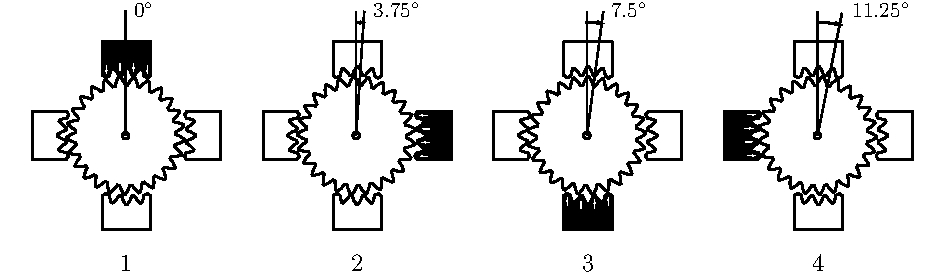
\includegraphics[width=1\textwidth]{diagrams/stepperMotor.pdf}
					\caption{Stepper motor operation}
					\label{fig:stepperMotor}
				\end{figure}
				
				By controlling these steps, the motor's rotation and speed can be
				exactly controlled. Stepper motors lack active feedback mechanisms and
				rely solely on the motor successfully completing every step. This
				assumption does not hold if the motor is unable to provide enough torque
				(turning power) to move its load. As a result, the motors used by the
				printer are designed to be powerful enough to reliably provide the
				torque needed so that sensors are not needed to judge the position of
				the system.
				
			\subsubsection{Extruder}
				
				The extruder uses a simple DC motor and gearbox to force a filament of
				acrylonitrile butadiene styrene (ABS) plastic, the material Lego is made
				from, into a heater and out of a fine nozzle (figure \ref{fig:extruder}).
				A temperature sensor is installed in the heater allowing the temperature
				to be carefully controlled to ensure an even flow.
				
				\begin{figure}
					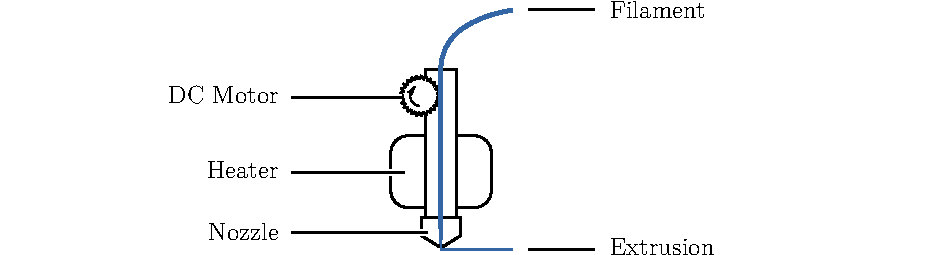
\includegraphics[width=1\textwidth]{diagrams/extruder.pdf}
					\caption{Extruder components}
					\label{fig:extruder}
				\end{figure}
				
			\subsubsection{Platform}
				
				The platform contains a heated build surface which  helps prevent prints
				warping and this also improves the adhesion of the print to the build surface.
				
				The build surface is also a conveyor belt powered by a small DC motor
				and gearbox. It is used to eject printed objects after printing
				completes allowing continuous printing operations.
				
		\subsection{Electronics}
		
			The Makerbot is controlled by the RepRap's generation 3 electronics
			\cite{reprapelectronics}. These
			consist of:
			\begin{description}
				
				\item[Motherboard] This circuit board hosts an 8-bit microcontroller
				which communicates with a computer via a custom serial interface and
				controls the printer's operation.
				
				\item[Extruder Controller] This circuit board hosts a second small
				microcontroller along with electronics for the extruder's motor and
				temperature sensor.  The extruder controller communicates with the
				motherboard via a custom RS485 interface.
				
				\item[Relay Board] This circuit board contains a mechanical relay for
				turning each of the two heaters on and off. The relay board is driven by
				the extruder controller using simple digital signals.
				
				\item[Stepper Motor Driver ($\times 3$)] Circuit boards which produce
				the high-power signals required to drive the stepper motors. These
				boards are connected to the motherboard via a simple digital interface
				that abstracts away many of the electrical and timing difficulties
				driving a stepper motor.
				
			\end{description}
	
		\subsection{Microcontrollers}
			
			The electronics use a pair of Arduino-compatible microcontrollers to drive
			the printer. These devices have a fairly minimal 8-bit instruction set,
			limited amounts of memory (4KB of RAM) and a very limited set of options
			for high-speed communications. A faster microcontroller capable of faster
			communication and command processing is needed to solve the performance
			problems described in \S\ref{sec:aims}.
		
		\subsection{Firmware}
			
			The firmware on the microcontrollers is responsible for two main tasks:
			receiving print data from a computer and producing the signals required
			for printing. The signals produced have strict `real-time' timing
			requirements and so to meet these, specialised timing hardware within the
			microcontroller must be used.
			
			3D printers typically receive print data in the form of G-code files
			\cite{reprapgcode}. G-code is the de facto standard for controlling
			computer numerical control (CNC) machines such as 3D printers, laser
			cutters and lathes. The language is human readable and defines
			step-by-step instructions for machine actions such as `move to (X,Y,Z)' or
			`enable heater'.
			
			The RepRap generation 3 firmware on the motherboard uses a custom serial
			protocol to communicate with the host computer. This protocol is designed
			to be simple for the microcontroller to use and, as well as various
			diagnostic features contains a compressed version of G-code.
			
		\subsection{G-Code}
			
			\label{sec:gcodemachine}
			
			G-code is assumed to execute on an abstract `G-code machine'. The machine
			consists of 26 numeric registers named `A' to `Z'.  A G-code instruction
			consists of a set of register assignments after which the machine
			executes a specific action based on the contents of its registers.
			
			Some registers may be reset to an `undefined' state before each
			instruction allowing the machine to identify when a register is written.
			For example, the `G' and `M' registers are used to specify what type of
			action should occur and, if not cleared, it would be impossible
			to determine which register contains the action required.
			
			Each register accepts either a floating point or integer value, for
			example the `G' and `M' registers only accept integer action numbers while
			`X', `Y' and `Z' are floating point and accept coordinates.
			
			For example, when the instruction \verb|G1 X10 Y-15 Z0.3 F3000| is encountered,
			the following register values are set:
			
			\begin{gcoderegs}
				\reg{F}{3000}
				\reg{G}{1}
				\reg{X}{10}
				\reg{Y}{-15}
				\reg{Z}{0.3}
			\end{gcoderegs}
			
			In this example, the action is determined based on the `G' register to be
			`move to' and the `X', `Y' and `Z' registers determine where to move and
			`F' at what speed. If this is followed by \verb|M104 S225| then the
			following registers will be set:
			
			\begin{gcoderegs}
				\reg{F}{3000}
				\reg{M}{104}
				\reg{S}{225}
				\reg{X}{10}
				\reg{Y}{-15}
				\reg{Z}{0.3}
			\end{gcoderegs}
			
			Note that the `G' register has been undefined but the others have
			remained. In this example, the action is determined based on the `M'
			register to be `set extruder temperature' and the `S' register determines
			the temperature. `X', `Y', `Z' and `F' are ignored. Finally, if
			\verb|G1 Z0.6| is encountered the following registers are set:
			
			\begin{gcoderegs}
				\reg{F}{3000}
				\reg{G}{1}
				\reg{S}{225}
				\reg{X}{10}
				\reg{Y}{-15}
				\reg{Z}{0.6}
			\end{gcoderegs}
			
			Once again the machine determines the action to be `move to' and moves to
			the position defined by `X', `Y' and `Z' at the speed in `F', ignoring the
			`S' register.  Because the values of `X', `Y' have not been changed, the
			machine will move only the `Z' axis.
		
		\subsection{Support Software}
			
			The G-code used by the printer is generated from 3D models using an
			open-source tool called Skeinforge \cite{skeinforge}. Skeinforge is
			typically used as part of ReplicatorG, a graphical user interface for
			preparing and printing 3D models \cite{replicatorg}. ReplicatorG can also
			handle the translation of G-code into the compressed format used by the
			RepRap firmware.  Other less mature tools, such as Slic3r, are available
			but less frequently used.
		
	\section{ARM \& Mbed}
		
		As well as high-performance processors designed for phones, ARM also design
		the Cortex-M series of microcontrollers. For this project a Cortex-M3 based
		`Mbed' microcontroller was chosen to replace the pair of existing 8-bit
		microcontrollers \cite{mbed}. The reasons for the suitability of this choice
		are justified in this section.
		
		\subsection{Mbed}
			
			The Mbed is a small microcontroller prototyping board centred around the
			NXP LPC1768, ARM Cortex-M3 based microcontroller (figure \ref{fig:mbed}).
			It has has four debugging LEDs, a USB port for loading programs various
			input/output facilities including facilities for attaching an Ethernet
			port. The pins on the device expose these input and output capabilities
			and fit into standard 0.1" spaced circuit boards and prototyping
			breadboards.
			
			\begin{figure}
				
\includegraphics[width=1\textwidth]{diagrams/mbed.pdf}
				\caption{Mbed microcontroller}
				\label{fig:mbed}
			\end{figure}
			
			The Mbed provides a USB flash drive-like interface. This interface is used
			to program the device by simply copying a binary file onto it. This
			mechanism is used to support the device's unusual choice of purely
			web-based official development tools. Web-based development was not ideal
			for this project and an alternative solution is discussed in
			\S\ref{sec:compiler} allowing conventional development tools to be used.
		
		\subsection{NXP LPC1768}
			
			The LPC1768 microcontroller behind the Mbed provides the ARM Cortex-M3
			processor with various useful peripherals. It runs at up to $100\MHz$ and
			has $32\KB$ of ram \cite{lpc1768}.  While still a seemingly tiny amount
			compared to even a modest smart phone, this is a large amount for a
			microcontroller without the overhead of running a fully-fledged general
			purpose operating system and associated software.
			
			The chip contains various peripherals such as hardware timers, analog
			interfaces and, importantly, fast Ethernet support. These timers will, as
			with the previous microcontrollers, be vital for driving the electronics
			properly. Analog inputs are also needed to interface with the electronics.
			Ethernet support will allow the microcontroller to quickly receive
			detailed print data over the network.
			
			As well as these features, ARM devices are widely used and boast mature,
			open-source development tools making it an ideal choice for expanding the
			open-source Makerbot design.
			
	\section{Real-Time Operating Systems}
		
		The firmware consists of various complimentary parts (such as communication
		and control), which are easily managed with the use of an operating system.
		Due to the absolute timing and performance requirements FreeRTOS, a
		real-time operating system (RTOS), was selected.
		
		\subsection{Differences With Non-Real-Time Systems}
			
			Real-time operating systems, like other operating systems, provides a
			scheduler which allows multiple processes to run as if simultaneously. It
			also provides facilities for communicating between these processes. Unlike
			regular operating systems, an RTOS can provide exact timing guarantees.
			They are also generally be targeted at microcontroller development with
			tight resource constraints and without the need for extra hardware such as
			a memory management unit (MMU).
			
		\subsection{FreeRTOS}
			
			FreeRTOS is a widely used, open-source RTOS designed for use with a range
			of microcontrollers, including many Cortex-M3 based devices
			\cite{freertos}. The two key features provided by FreeRTOS are `tasks' and
			`queues' which are described below.
			
			\subsubsection{Tasks}
				
				A system built on FreeRTOS can be structured as several tasks
				executing in parallel. Tasks are similar to processes or threads on a
				conventional operating system with each task having its own set of
				registers and a stack.
				
				Because the microcontroller can only run one task at once, the FreeRTOS
				uses preemptive scheduling to approximate this behaviour where the
				current task is periodically interrupted by a timer (preempted) and a
				different task put in its place. If tasks are switched fast enough, they
				appear to run simultaneously.
				
				Tasks may be given different priorities and can be suspended until
				events such as a timer expiring or a hardware resource becoming
				available occur. The timing of the operating system's actions can be
				guaranteed allowing real-time systems to be developed.
				
			\subsubsection{Queues \& Mutexes}
				
				To provide synchronisation and communication between tasks, FreeRTOS
				provides a queue structure. Queues are defined which allow data to be
				inserted or removed with a first-in-first-out (FIFO) access scheme.
				
				These queues can be used safely by multiple tasks simultaneously without
				race conditions and so are ideal for inter-task communication.  Because
				of this safety, they also form the basis for standard parallel
				programming constructions such as semaphores and mutexes.
				
				When accessing a FreeRTOS queue a task may become blocked, for example,
				when adding an item to a queue that is already full. FreeRTOS can
				provide timing guarantees on timeouts waiting for these functions to
				complete. It also allows a task's priority to be temporarily raised when
				resumed after a blocking call, ensuring it is scheduled as soon as
				possible, reducing the delay before any new data data is processed.
